\documentclass[UTF8,a4paper,12pt,fontset=fandol]{ctexart}

% ======================
% 页面与基础宏包
% ======================
\usepackage{geometry}
\geometry{left=2.5cm, right=2.5cm, top=2.8cm, bottom=2.8cm}

\usepackage{amsmath, amssymb}
\usepackage{graphicx}
\usepackage{booktabs}
\usepackage{float}
\usepackage{setspace}
\usepackage{xcolor}
\usepackage{caption}
\usepackage{subcaption}
\usepackage{listings}

% 不使用 hyperref，保证目录为纯文本
\setstretch{1.4}

% ======================
% 代码环境
% ======================
\lstset{
  language=Python,
  basicstyle=\ttfamily\small,
  keywordstyle=\color{blue},
  commentstyle=\color{gray},
  stringstyle=\color{red},
  breaklines=true,
  frame=single,
  numbers=left,
  numberstyle=\tiny
}

% ======================
% 标题信息
% ======================
\title{
  基于 AI 数据驱动的锂离子电池容量衰退预测研究\\
  \large —— 针对商用 18650 电池老化过程中的内在差异性分析
}
\author{
  第六组：周鹏程 \quad 朱冠儒\\
  指导教师：陈震 \quad 任品泽\\
  清华大学 \quad BDMI
}
\date{2025 年 12 月}

\begin{document}
\maketitle

% ======================
\begin{abstract}
锂离子电池作为电动汽车与电网储能系统的核心部件，其容量衰退行为直接影响系统安全性与经济性。
本文基于真实商用 18650 锂离子电池循环数据，构建了一套数据驱动的容量衰退预测框架，
对比分析了 Transformer、LSTM 与 XGBoost 等模型在长周期退化建模中的性能差异，
并进一步研究了小波变换等信号处理方法对模型预测结果的影响。
\end{abstract}

\newpage
\tableofcontents
\newpage

% ======================
\section{研究背景与意义}
% ======================

锂离子电池被广泛应用于电动汽车与电网级储能系统。
在工程应用中，单体电芯通常需要经过筛选并组成大规模电池系统。
尽管在出厂阶段可以通过容量与内阻等指标进行匹配，
但在长期循环与复杂工况下，电池仍会表现出显著的个体老化差异。

容量是表征电池健康状态（State of Health, SOH）的核心指标之一。
对于典型商用 18650 电池，其在约 1000 次循环后容量通常衰减至初始值的 50\%--60\%。
因此，发展高精度、可解释的容量衰退预测模型具有重要工程价值。
% ======================
\section{预测模型方法}
% ======================

在锂离子电池容量衰退预测问题中，
模型不仅需要具备较高的预测精度，
还需要能够刻画长时间尺度上的非线性退化趋势，
并对局部波动与突变保持一定敏感性。
基于上述需求，本文选取了三类具有代表性的预测模型，
分别从长序列建模、经典时序建模以及集成学习角度进行对比分析。

\subsection{Transformer 模型}

Transformer 模型基于自注意力（Self-Attention）机制，
通过显式建模任意时间步之间的依赖关系，
避免了传统递归结构在长序列建模中存在的梯度衰减问题。
在电池容量衰退预测任务中，
Transformer 能够同时关注早期循环特征与后期容量变化，
从而捕捉跨越数百甚至上千循环的全局退化趋势。

与传统时序模型相比，
Transformer 不依赖严格的时间递推结构，
可以并行处理整个循环序列，
在复杂非线性退化路径建模方面具有明显优势。
因此，本文将 Transformer 作为主要研究对象，
用于评估其在长期容量衰退预测中的性能表现。

\subsection{LSTM 模型}

LSTM（Long Short-Term Memory）是一种经典的循环神经网络结构，
通过引入遗忘门、输入门和输出门机制，
在一定程度上缓解了普通 RNN 在长序列训练中的梯度消失问题。
其优势在于对时间顺序信息的自然建模能力，
在中短期时序预测任务中表现稳定。

然而，在电池容量衰退这一典型的超长序列问题中，
LSTM 仍然主要依赖逐步状态传递来存储历史信息，
其对远距离依赖关系的刻画能力有限。
这使得 LSTM 在捕捉长期退化趋势和全局演化规律时，
往往更关注局部平均行为，
对容量突变前的先兆特征响应相对不足。

\subsection{XGBoost 模型}

XGBoost 属于梯度提升决策树（GBDT）模型，
通过不断拟合前一轮模型的残差来提升整体预测精度。
该模型不直接依赖时间递推结构，
而是将容量衰退问题视为输入特征到输出容量之间的非线性映射。

在本研究中，
XGBoost 主要用于验证基于统计特征的传统机器学习方法
在容量衰退预测任务中的适用性。
其优势在于训练速度快、对异常值和噪声具有较强鲁棒性，
但在面对连续、平滑且具有长期相关性的退化过程时，
对整体趋势的刻画能力相对有限。

\subsection{模型选择与对比思路}

通过引入上述三类模型，
本文从不同建模范式出发，
系统比较了深度学习模型与传统集成学习方法
在电池容量衰退预测任务中的表现差异。
这种对比有助于明确：
在复杂、长周期退化问题中，
不同模型结构在捕捉长期趋势、局部波动以及预测稳定性方面的优劣特性。

% ======================
\section{实验结果与模型效果}
% ======================

\subsection{不同模型预测效果对比}

\begin{figure}[H]
  \centering
  \begin{subfigure}{0.45\linewidth}
    \centering
    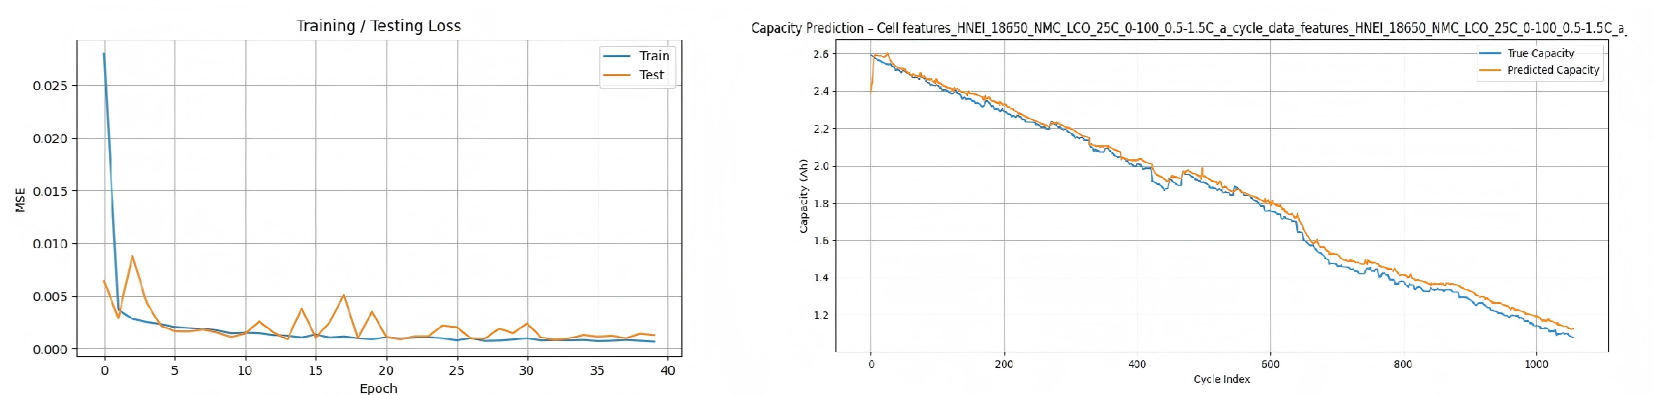
\includegraphics[width=\linewidth]{fig/slide-11.png}
    \caption{Transformer 预测结果}
  \end{subfigure}
  \hfill
  \begin{subfigure}{0.45\linewidth}
    \centering
    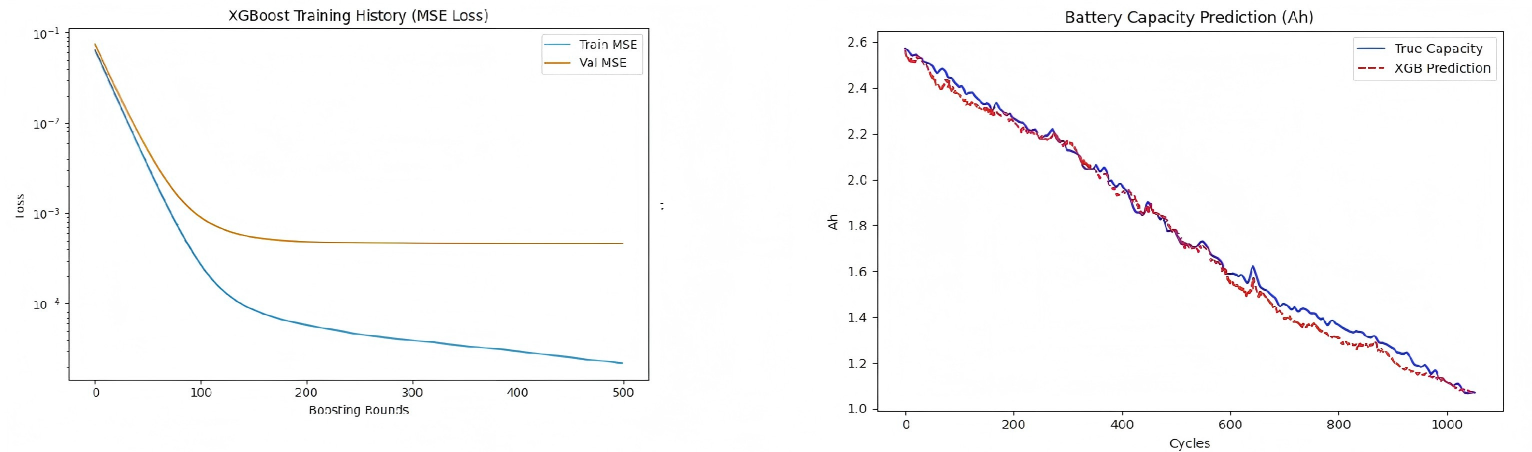
\includegraphics[width=\linewidth]{fig/slide-12.png}
    \caption{XGBoost 预测结果}
  \end{subfigure}
  \caption{不同模型在容量衰退预测任务中的效果对比}
\end{figure}

\noindent\textbf{LSTM 模型结果描述：}  
LSTM 模型在训练初期表现出较快的收敛速度，
训练与测试损失整体趋势一致，
最终均方误差稳定在 $10^{-3}$ 量级。
然而，在容量衰退速率发生变化或出现局部波动的区段，
其预测结果表现出一定的过度平滑特征，
对突变前的先兆信息响应不足。

% ======================
\section{小波变换影响分析}
% ======================

\begin{figure}[H]
  \centering
  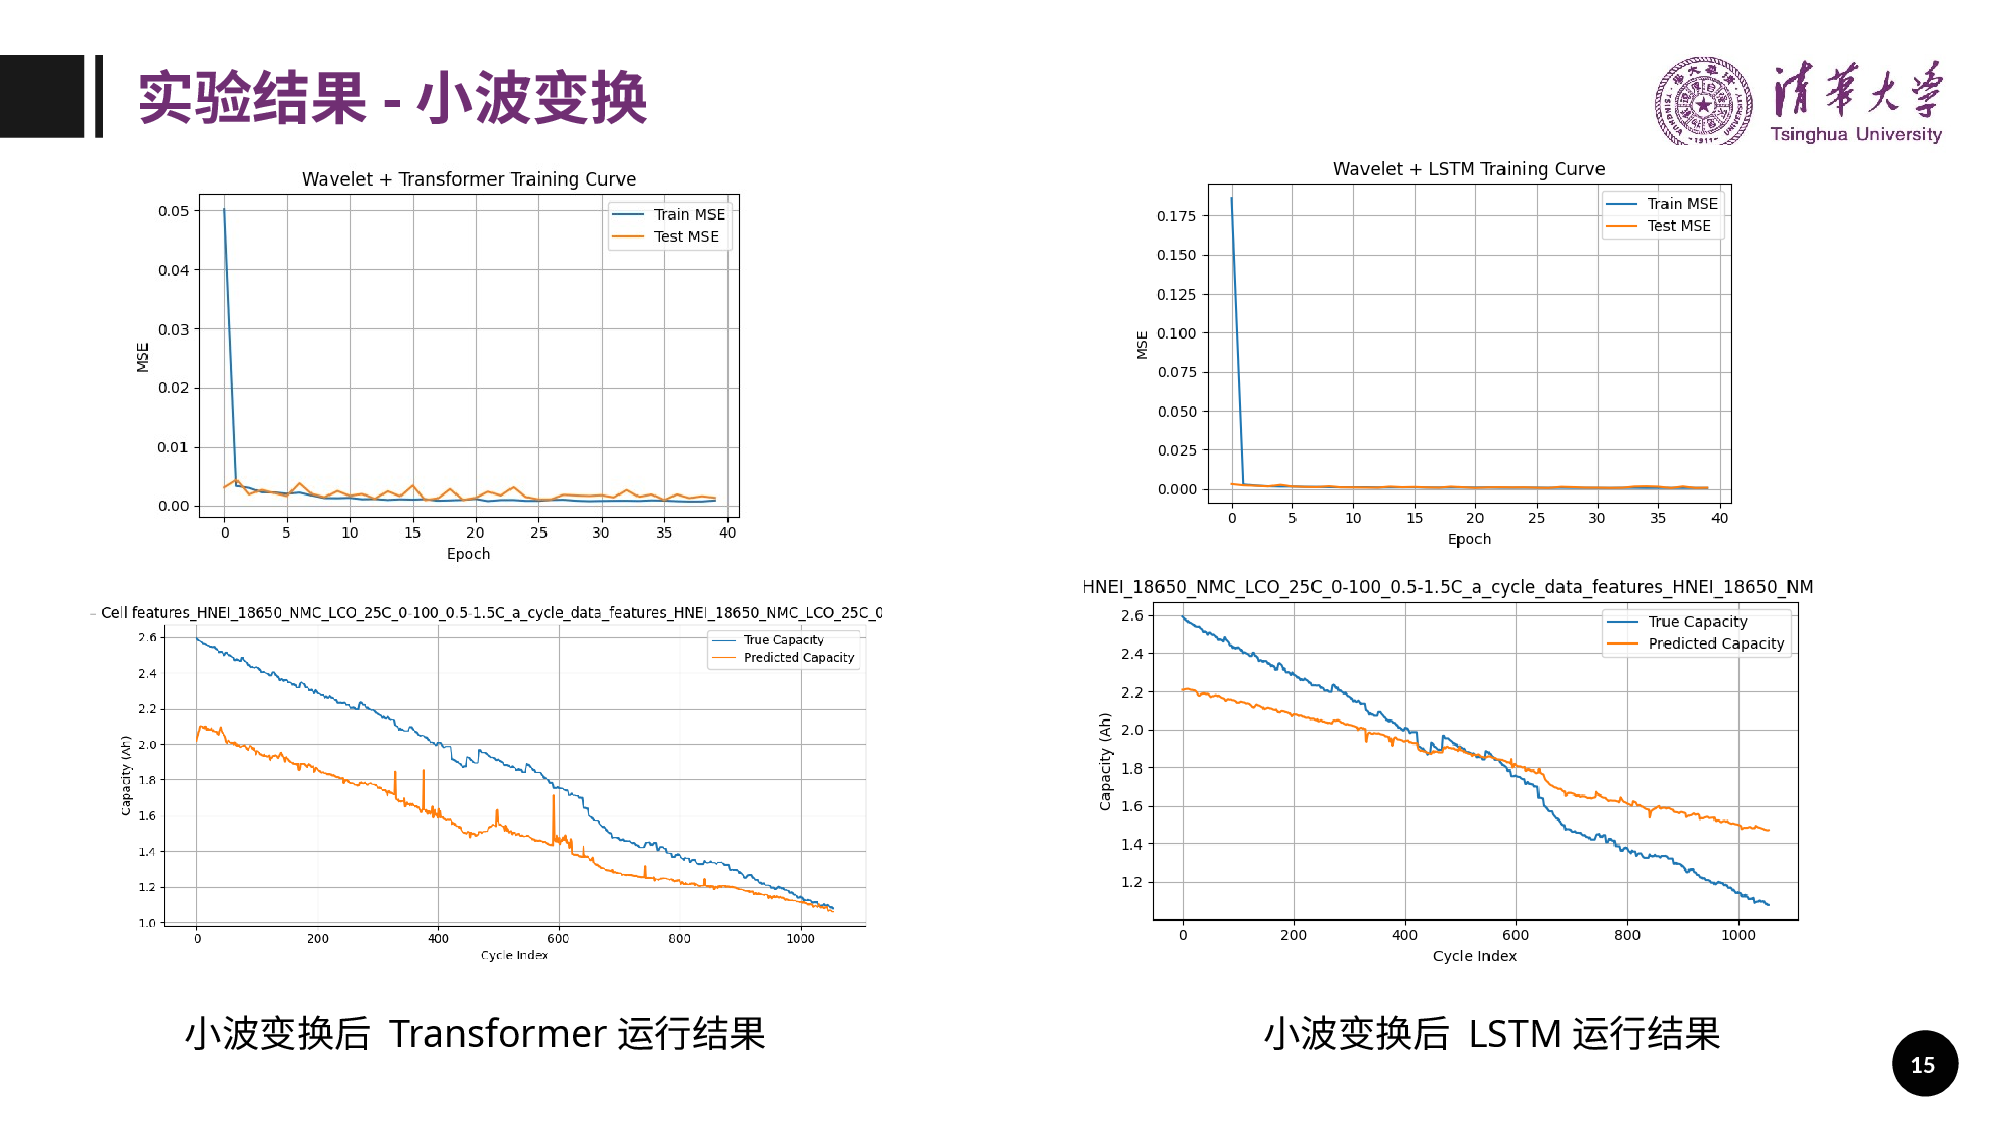
\includegraphics[width=0.95\linewidth]{fig/slide-14.png}
  \caption{小波变换后 Transformer 与 LSTM 的预测结果对比}
\end{figure}

实验结果表明，小波变换在降低预测方差的同时，
可能引入系统性偏差。
对于 LSTM 模型，小波处理相当于双重平滑，
削弱了容量骤降前的微弱先兆信息；
对于 Transformer，小波重构可能导致信号均值或尺度发生偏移，
从而使预测结果整体偏低。

% ======================
\section{结论与未来展望}
% ======================

本文基于真实循环数据，系统比较了多种数据驱动模型在锂离子电池容量衰退预测任务中的表现。
实验结果表明，Transformer 在长期趋势建模方面具有显著优势，
而传统时序模型与集成学习方法在复杂退化路径下仍存在一定局限。

\subsection*{未来展望}

未来研究可从以下几个方面进一步展开：

\begin{itemize}
  \item \textbf{引入物理信息约束的混合模型：}
  纯数据驱动模型在外推能力和可解释性方面仍存在不足。
  后续可将电化学机理、内阻增长规律或能量守恒关系
  以物理约束或正则项的形式引入模型训练过程，
  构建物理信息引导的深度学习框架。

  \item \textbf{面向在线预测的轻量化建模：}
  Transformer 虽然预测精度高，但计算复杂度较大。
  未来可探索模型剪枝、知识蒸馏或滑动窗口注意力机制，
  以提升模型在电池管理系统（BMS）中的实时部署能力。

  \item \textbf{更精细的退化阶段建模：}
  电池衰退过程通常具有明显的阶段性特征。
  后续可将容量退化划分为不同阶段，
  并结合阶段识别模型实现分阶段预测，
  以提高对容量突变和加速退化区段的预测准确性。
\end{itemize}

\section*{致谢}
感谢指导教师在研究过程中的耐心指导与宝贵建议。

\end{document}
